\documentclass[10pt]{beamer}
\usetheme{pohan}
\usepackage{lipsum}
\usepackage{tabularx}
\usepackage{xcolor}
\usepackage{fancybox, graphicx}
\usepackage{animate}
\usepackage{subcaption}


\renewcommand{\arraystretch}{2}
\renewcommand\tabularxcolumn[1]{m{#1}}
\title{7/9 Paper Intro}
\subtitle{}
\author{Pohan Chi}
\date{\today}


\begin{document}

\maketitle

\maketoc

\section{Contextualized Sparse Representations for
Real-Time Open-Domain Question Answering}

\section{Pretraining with Contrastive Sentence Objectives Improves Discourse Performance of Language Models}

\section{Transformers are RNNs: Fast Autoregressive Transformers with Linear Attention}

\begin{frame}{Open-Domain QA}
    \begin{figure}
        \begin{center}
            \shadowbox{\includegraphics[width=0.96\textwidth]{img/opendomain}}
        \end{center}
    \end{figure}
    \begin{center}
        \shadowbox{Accepted by ACL 2020}
    \end{center}
\end{frame}

\begin{frame}{Open-Domain QA}
   Overview
   \begin{itemize}
    \item Task definition
    \item Motivation
    \item Methodology
    \item Experiments
    \item Conclusion
   \end{itemize}
\end{frame}

\begin{frame}{Open-domain QA}
    \begin{figure}
        \begin{center}
            Task Definition - DrQA
            \vfill
            \shadowbox{\includegraphics[width=0.7\textwidth]{img/environment}}
            \vfill
            Given all full wikipedia documents, answer the question.
        \end{center}
    \end{figure}
\end{frame}

\begin{frame}{One solution: BM25 + RC-Model}
    \begin{figure}
        
    \end{figure}
\end{frame}

\begin{frame}[t]{Sentence Representation}

    \begin{figure}
        \begin{center}
            \shadowbox{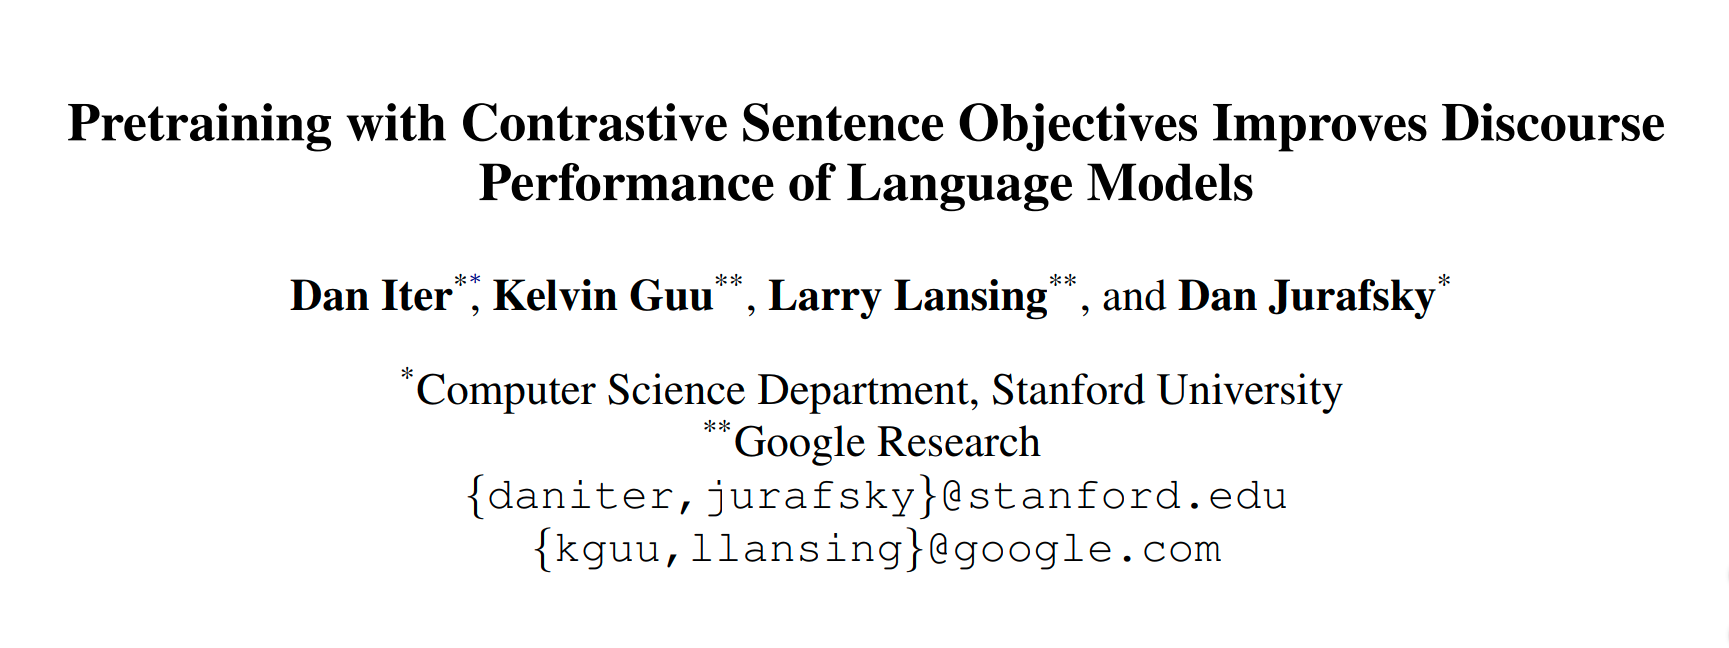
\includegraphics[width=0.96\textwidth]{img/predictive}}
        \end{center}
    \end{figure}
    \begin{center}
        \shadowbox{Accepted by ACL 2020}
    \end{center}
\end{frame}

\begin{frame}{Highlight}

    \begin{itemize}
        \item sentence-level CPC objective + MLM loss in pretraining stage
        \item Compare to SOP and NSP Pretraining Method
    \end{itemize}

\end{frame}

\begin{frame}{Overview}

Overview
\begin{itemize}
    \item Task Definitions
    \item Evaluation
    \item Methodology \& Model
    \item Experiments
    \item Conclusion
\end{itemize}

\end{frame}

\begin{frame}[t]{Sentence Representation}

    \begin{figure}
        \begin{center}
            \shadowbox{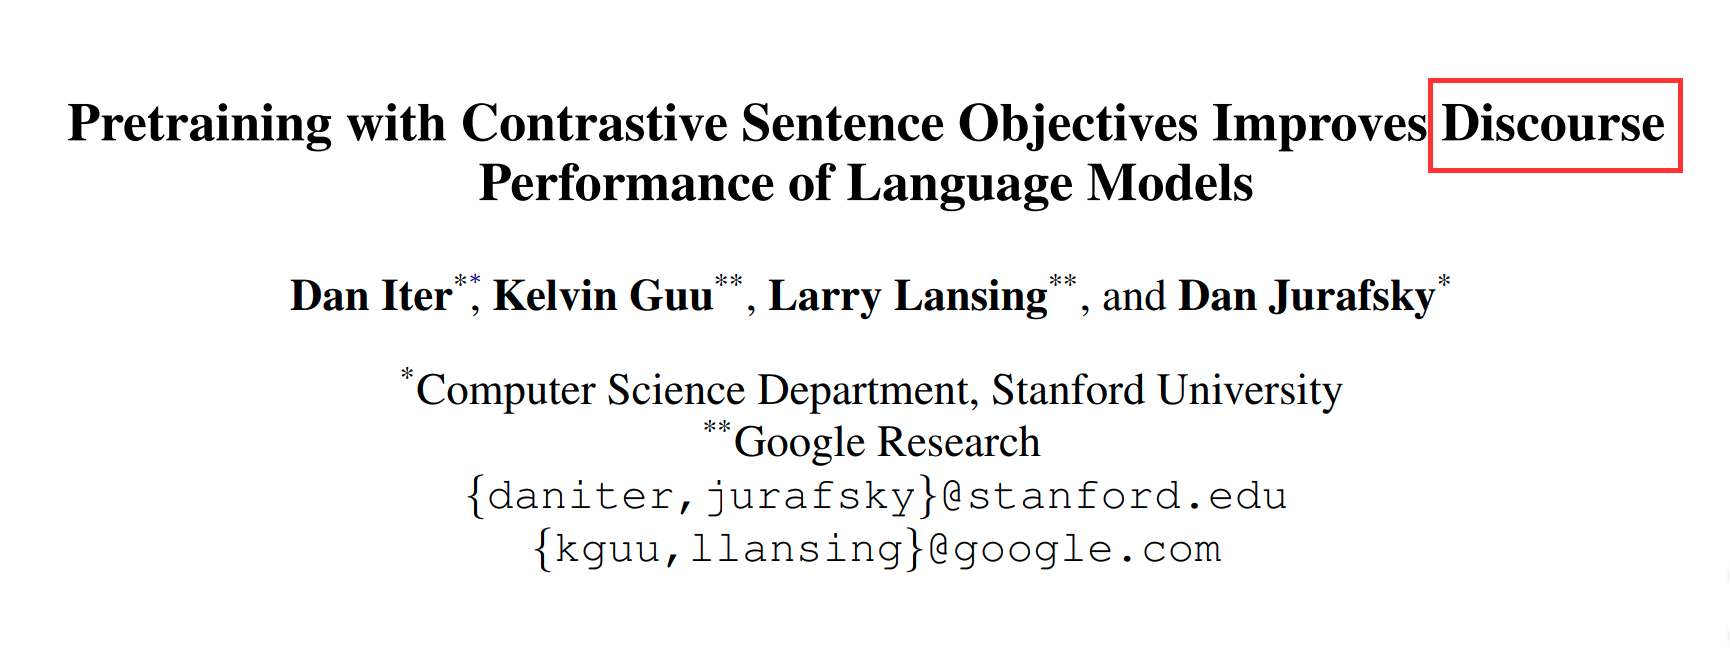
\includegraphics[width=0.96\textwidth]{img/reference}}
        \end{center}
    \end{figure}
    \begin{center}
        \shadowbox{Accepted by ACL 2020}
    \end{center}
\end{frame}

\begin{frame}{Task Definitions}
    Discourse 
    \begin{itemize}
        \item Discourse is a coherent structured group of sentence 
        \item ex: dialogue, document
    \end{itemize}

    ex: 

    \begin{figure}
        \begin{center}
            \shadowbox{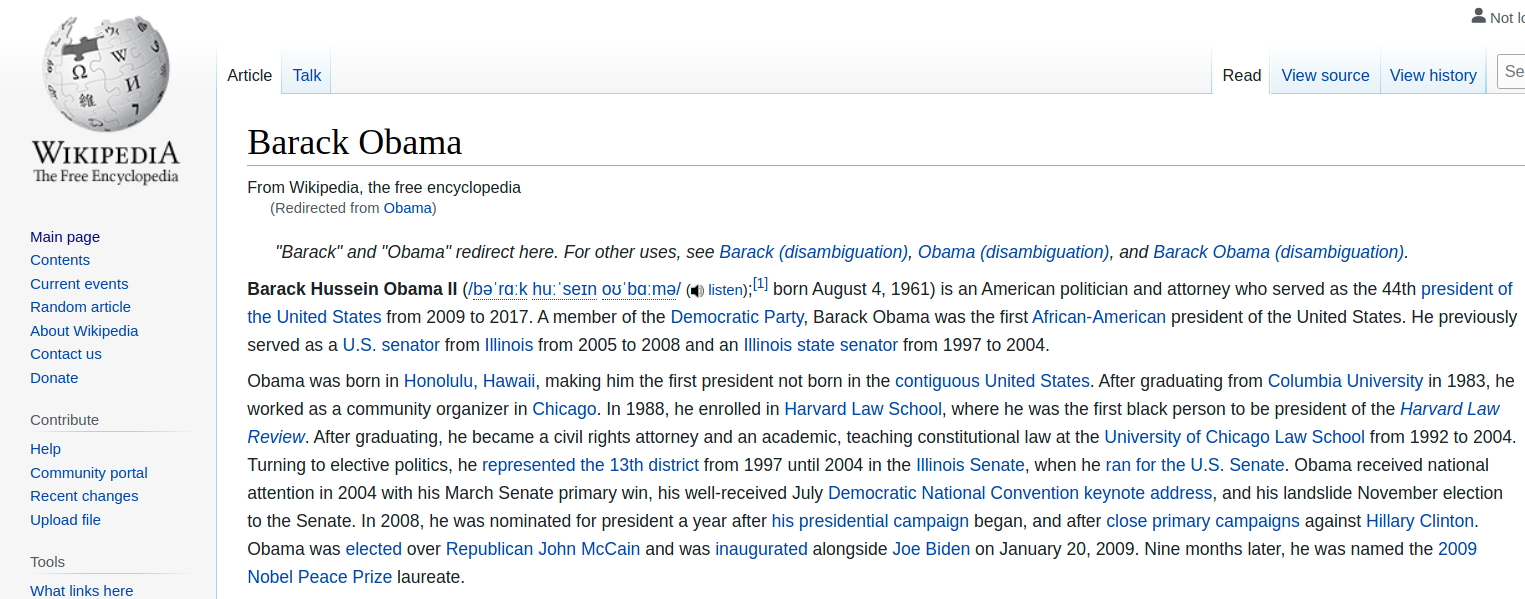
\includegraphics[width=0.96\textwidth]{img/obama_example}}
        \end{center}
    \end{figure}

\end{frame}

\begin{frame}{Discourse Evaluation}

    \begin{itemize}
        \item Sentence Position (SP)
        \item BSO (Binary Sentence Ordering) (same as SOP)
        \item DC (Discourse Coherence)
        \item SSP (Sentence Section Prediction)
        \item PDTB-E, PDTB-I, RST-DT
    \end{itemize}

\end{frame}

\begin{frame}{Model \& Objectives}
    \begin{figure}
        \begin{center}
            \shadowbox{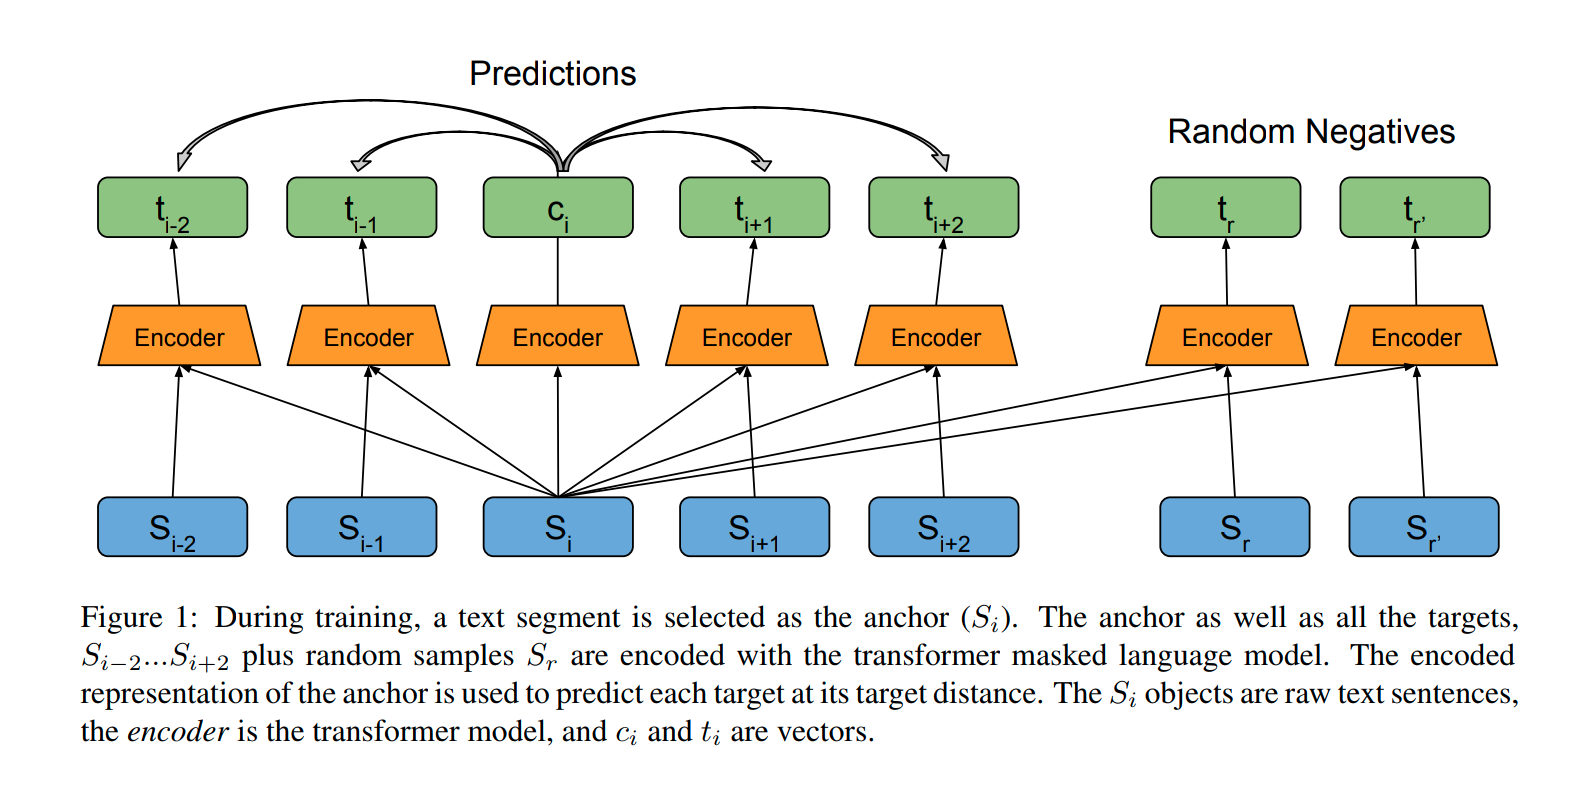
\includegraphics[width=0.96\textwidth]{img/cpc_model}}
        \end{center}
    \end{figure}
\end{frame}

\begin{frame}{Experiments - 1}
    \begin{figure}
        \begin{center}
            \shadowbox{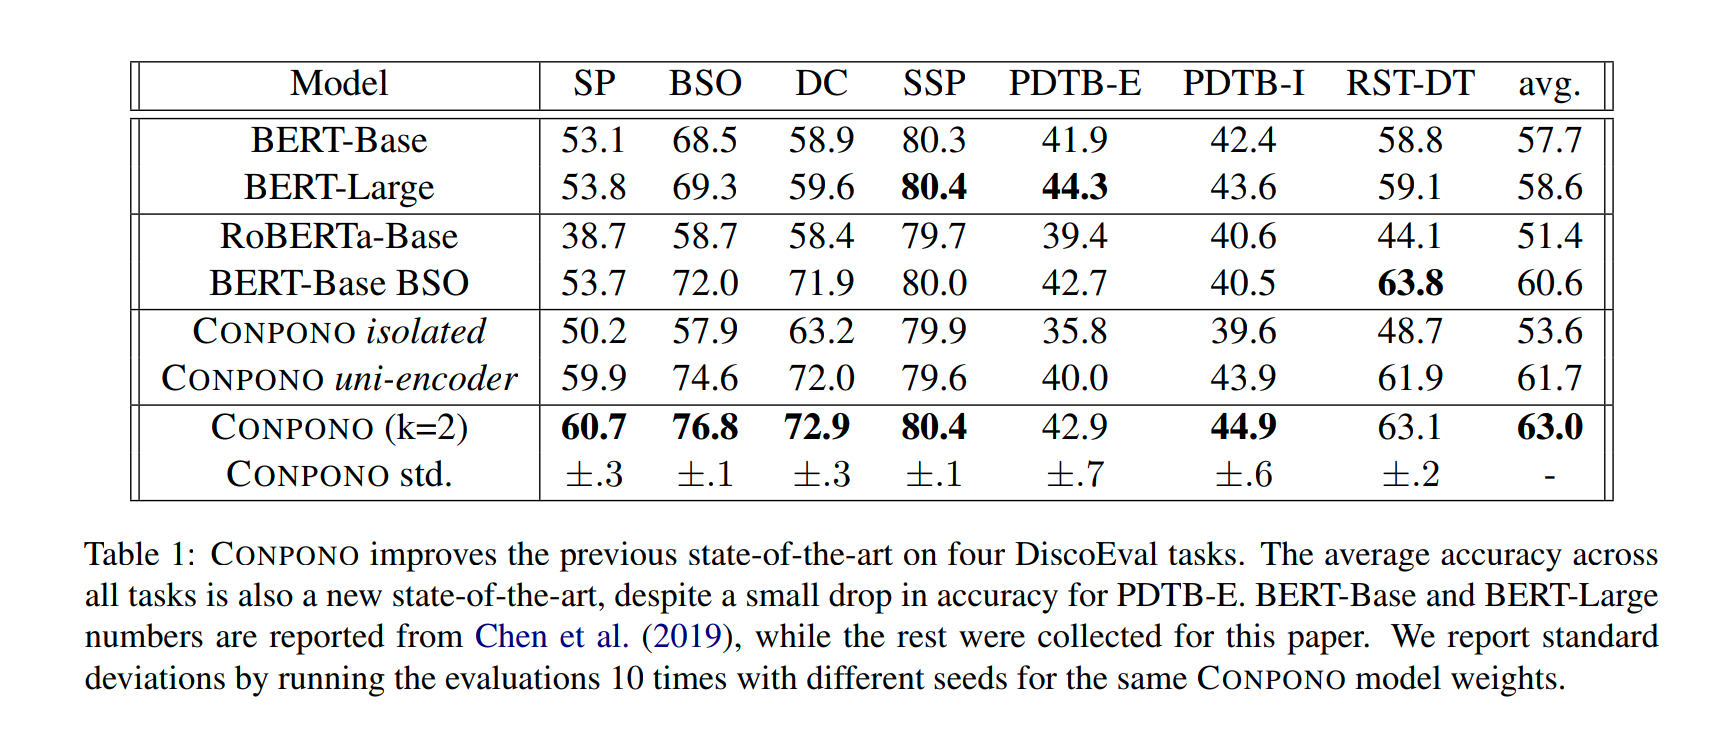
\includegraphics[width=0.96\textwidth]{img/results}}
        \end{center}
    \end{figure}
\end{frame}


\begin{frame}{Experiments - 2}
    \begin{figure}
        \begin{subfigure}{.5\textwidth}
            \centering
            \shadowbox{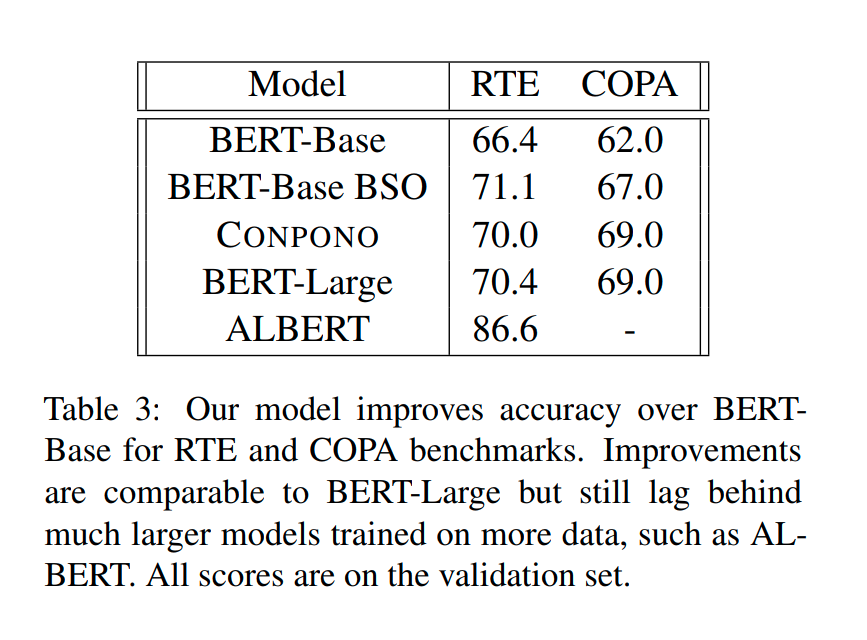
\includegraphics[width=.9\linewidth]{img/readingComprehension}}
        \end{subfigure}%
        \begin{subfigure}{.5\textwidth}
            \centering
            \shadowbox{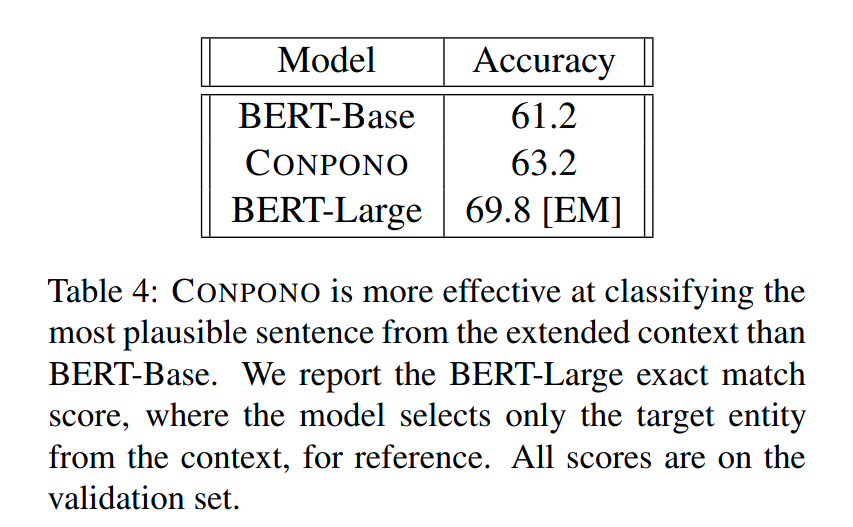
\includegraphics[width=.9\linewidth]{img/reading}}
        \end{subfigure} 
    \end{figure}
\end{frame}

\begin{frame}{Conclusion \& A lot}
    \begin{itemize}
        \item benchmark in DiscoEval (sentence representation) 
        \item Also improve performance in RTE, COPA, ReCoRD (Reading Comprehension).
        \item uni-encoder verse isolated coding comparison
    \end{itemize}
\end{frame}

\begin{frame}[t]{Linear Attention}

    \begin{figure}
        \begin{center}
            \shadowbox{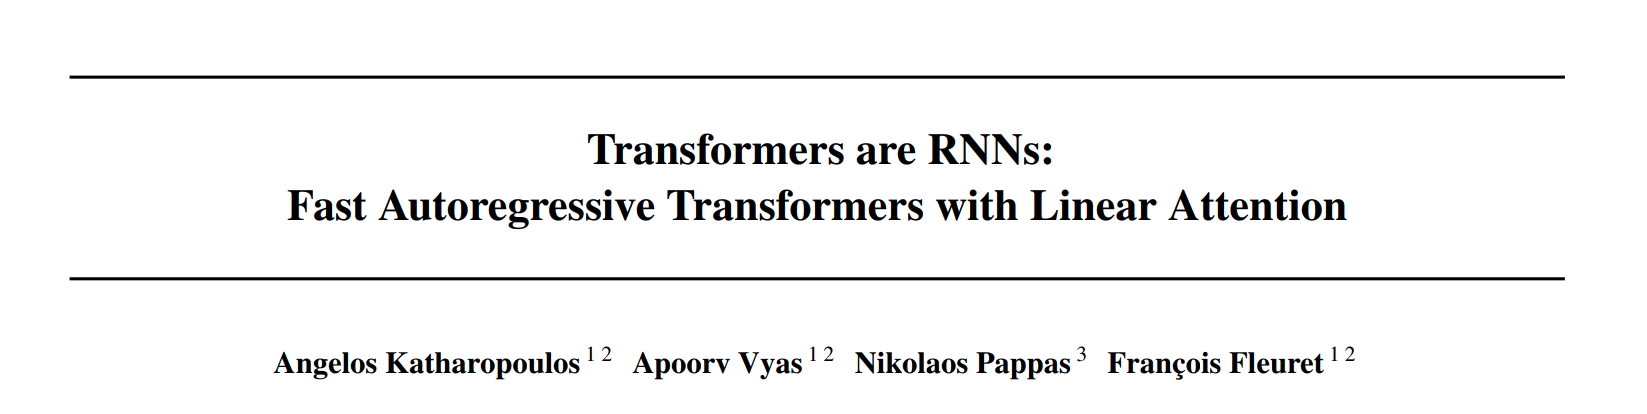
\includegraphics[width=0.96\textwidth]{img/transformer_RNN}}
        \end{center}
    \end{figure}
    \begin{center}
        \shadowbox{Accepted by ICML 2020}
    \end{center}
\end{frame}

\begin{frame}{Highlight}

    \begin{itemize}
        \item Reduce $O(N^2)$ to $O(N)$ 
        \item Connect Transformer to RNN form
        \item Compare to Reformer (LSH attention)
    \end{itemize}

\end{frame}

\begin{frame}{Overview}

Overview
\begin{itemize}
    \item Refomulate Equation
    \item Experiments
    \item Conclusion
\end{itemize}

\end{frame}

\begin{frame}{Self attention}

    Original

    \begin{figure}
        \begin{center}
            \shadowbox{\includegraphics[height=0.6\textheight]{img/self_att}}
        \end{center}
    \end{figure}
    link: https://www.idiap.ch/~katharas/pdfs/linear-transformers-slides.pdf
\end{frame}

\begin{frame}{Replace by arbitrary similarity score}

    \begin{figure}
        \begin{center}
            \shadowbox{\includegraphics[width=0.8\textwidth]{img/sim}}
        \end{center}
    \end{figure}
    link: https://www.idiap.ch/~katharas/pdfs/linear-transformers-slides.pdf
\end{frame}

\begin{frame}{kernalization - (1)}

    \begin{figure}
        \begin{center}
            \shadowbox{\includegraphics[width=0.8\textwidth]{img/sim_kernal}}
        \end{center}
    \end{figure}
    link: https://www.idiap.ch/~katharas/pdfs/linear-transformers-slides.pdf
\end{frame}

\begin{frame}{kernalization - (2)}

    \begin{figure}
        \begin{center}
            \shadowbox{\includegraphics[width=0.8\textwidth]{img/kernal-2}}
        \end{center}
    \end{figure}
    link: https://www.idiap.ch/~katharas/pdfs/linear-transformers-slides.pdf
\end{frame}

\begin{frame}{kernalization - (3)}

    \begin{figure}
        \begin{center}
            \shadowbox{\includegraphics[width=0.8\textwidth]{img/kernal-3}}
        \end{center}
    \end{figure}
    link: https://www.idiap.ch/~katharas/pdfs/linear-transformers-slides.pdf
\end{frame}

\begin{frame}{RNNs - (1)}

    \begin{figure}
        \begin{center}
            \shadowbox{\includegraphics[width=0.8\textwidth]{img/rnn}}
        \end{center}
    \end{figure}
    link: https://www.idiap.ch/~katharas/pdfs/linear-transformers-slides.pdf
\end{frame}

\begin{frame}{RNNs - (2)}

    \begin{figure}
        \begin{center}
            \shadowbox{\includegraphics[width=0.8\textwidth]{img/rnn2}}
        \end{center}
    \end{figure}
    link: https://www.idiap.ch/~katharas/pdfs/linear-transformers-slides.pdf
\end{frame}

\end{document}
